
\documentclass{standalone}
\usepackage{tikz}
\usetikzlibrary{arrows.meta,decorations.pathmorphing}

\begin{document}
\tikzset{every picture/.style={line width=0.75pt}} %set default line width to 0.75pt        

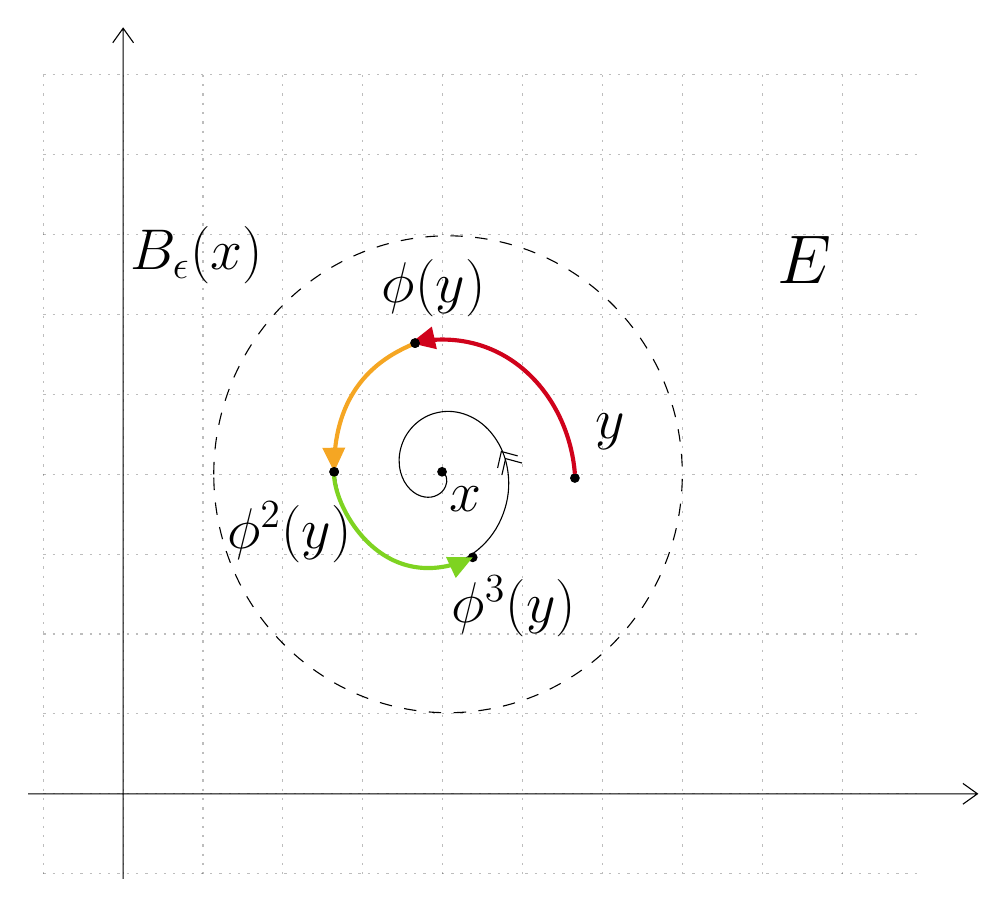
\begin{tikzpicture}[x=0.75pt,y=0.75pt,yscale=-1,xscale=1]
%uncomment if require: \path (0,446); %set diagram left start at 0, and has height of 446

%Shape: Axis 2D [id:dp5958965788842521] 
\draw  (26,374.85) -- (483.33,374.85)(71.73,6) -- (71.73,415.83) (476.33,369.85) -- (483.33,374.85) -- (476.33,379.85) (66.73,13) -- (71.73,6) -- (76.73,13)  ;
%Shape: Grid [id:dp9524606760405594] 
\draw  [draw opacity=0][dash pattern={on 0.84pt off 2.51pt}] (33.25,28.48) -- (456.59,28.48) -- (456.59,413.42) -- (33.25,413.42) -- cycle ; \draw  [color={rgb, 255:red, 0; green, 0; blue, 0 }  ,draw opacity=0.26 ][dash pattern={on 0.84pt off 2.51pt}] (33.25,28.48) -- (33.25,413.42)(71.73,28.48) -- (71.73,413.42)(110.22,28.48) -- (110.22,413.42)(148.7,28.48) -- (148.7,413.42)(187.19,28.48) -- (187.19,413.42)(225.67,28.48) -- (225.67,413.42)(264.16,28.48) -- (264.16,413.42)(302.64,28.48) -- (302.64,413.42)(341.13,28.48) -- (341.13,413.42)(379.62,28.48) -- (379.62,413.42)(418.1,28.48) -- (418.1,413.42) ; \draw  [color={rgb, 255:red, 0; green, 0; blue, 0 }  ,draw opacity=0.26 ][dash pattern={on 0.84pt off 2.51pt}] (33.25,28.48) -- (456.59,28.48)(33.25,66.97) -- (456.59,66.97)(33.25,105.45) -- (456.59,105.45)(33.25,143.94) -- (456.59,143.94)(33.25,182.42) -- (456.59,182.42)(33.25,220.91) -- (456.59,220.91)(33.25,259.39) -- (456.59,259.39)(33.25,297.88) -- (456.59,297.88)(33.25,336.36) -- (456.59,336.36)(33.25,374.85) -- (456.59,374.85)(33.25,413.34) -- (456.59,413.34) ; \draw  [color={rgb, 255:red, 0; green, 0; blue, 0 }  ,draw opacity=0.26 ][dash pattern={on 0.84pt off 2.51pt}]  ;
%Shape: Ellipse [id:dp48854496675935066] 
\draw  [dash pattern={on 4.5pt off 4.5pt}] (115.39,220.91) .. controls (115.39,157.46) and (165.92,106.02) .. (228.26,106.02) .. controls (290.6,106.02) and (341.13,157.46) .. (341.13,220.91) .. controls (341.13,284.36) and (290.6,335.79) .. (228.26,335.79) .. controls (165.92,335.79) and (115.39,284.36) .. (115.39,220.91) -- cycle ;
%Shape: Circle [id:dp7149274459952493] 
\draw  [fill={rgb, 255:red, 0; green, 0; blue, 0 }  ,fill opacity=1 ] (223.33,219.71) .. controls (223.33,218.57) and (224.25,217.65) .. (225.39,217.65) .. controls (226.52,217.65) and (227.44,218.57) .. (227.44,219.71) .. controls (227.44,220.84) and (226.52,221.76) .. (225.39,221.76) .. controls (224.25,221.76) and (223.33,220.84) .. (223.33,219.71) -- cycle ;
%Shape: Circle [id:dp7171311598003665] 
\draw  [fill={rgb, 255:red, 0; green, 0; blue, 0 }  ,fill opacity=1 ] (210.33,157.71) .. controls (210.33,156.57) and (211.25,155.65) .. (212.39,155.65) .. controls (213.52,155.65) and (214.44,156.57) .. (214.44,157.71) .. controls (214.44,158.84) and (213.52,159.76) .. (212.39,159.76) .. controls (211.25,159.76) and (210.33,158.84) .. (210.33,157.71) -- cycle ;
%Shape: Circle [id:dp2525359311831692] 
\draw  [fill={rgb, 255:red, 0; green, 0; blue, 0 }  ,fill opacity=1 ] (238.1,260.93) .. controls (238.1,259.8) and (239.02,258.88) .. (240.16,258.88) .. controls (241.29,258.88) and (242.22,259.8) .. (242.22,260.93) .. controls (242.22,262.07) and (241.29,262.99) .. (240.16,262.99) .. controls (239.02,262.99) and (238.1,262.07) .. (238.1,260.93) -- cycle ;
%Shape: Circle [id:dp19254067806539155] 
\draw  [fill={rgb, 255:red, 0; green, 0; blue, 0 }  ,fill opacity=1 ] (287.33,222.71) .. controls (287.33,221.57) and (288.25,220.65) .. (289.39,220.65) .. controls (290.52,220.65) and (291.44,221.57) .. (291.44,222.71) .. controls (291.44,223.84) and (290.52,224.76) .. (289.39,224.76) .. controls (288.25,224.76) and (287.33,223.84) .. (287.33,222.71) -- cycle ;
%Shape: Circle [id:dp22569853940877072] 
\draw  [fill={rgb, 255:red, 0; green, 0; blue, 0 }  ,fill opacity=1 ] (171.33,219.71) .. controls (171.33,218.57) and (172.25,217.65) .. (173.39,217.65) .. controls (174.52,217.65) and (175.44,218.57) .. (175.44,219.71) .. controls (175.44,220.84) and (174.52,221.76) .. (173.39,221.76) .. controls (172.25,221.76) and (171.33,220.84) .. (171.33,219.71) -- cycle ;
%Shape: Spiral [id:dp33651871858230575] 
\draw  [color={rgb, 255:red, 0; green, 0; blue, 0 }  ,draw opacity=1 ] (225.47,219.71) .. controls (226.45,220.17) and (227.12,221.05) .. (227.47,222.34) .. controls (227.85,223.77) and (227.71,225.26) .. (227.04,226.8) .. controls (226.28,228.52) and (225.05,229.86) .. (223.33,230.8) .. controls (221.41,231.87) and (219.3,232.21) .. (216.99,231.84) .. controls (214.43,231.43) and (212.12,230.2) .. (210.06,228.17) .. controls (207.8,225.94) and (206.24,223.12) .. (205.37,219.71) .. controls (204.43,216) and (204.47,212.21) .. (205.49,208.34) .. controls (206.6,204.15) and (208.67,200.54) .. (211.71,197.49) .. controls (214.98,194.21) and (218.85,192.1) .. (223.33,191.14) .. controls (228.11,190.1) and (232.86,190.55) .. (237.59,192.44) .. controls (242.6,194.45) and (246.84,197.81) .. (250.31,202.51) .. controls (253.97,207.47) and (256.24,213.21) .. (257.12,219.71) .. controls (258.05,226.55) and (257.3,233.25) .. (254.88,239.82) .. controls (252.35,246.71) and (248.34,252.45) .. (242.87,257.07) .. controls (237.15,261.89) and (230.63,264.79) .. (223.33,265.76) .. controls (215.72,266.78) and (208.33,265.56) .. (201.16,262.12) .. controls (193.71,258.53) and (187.53,253.04) .. (182.65,245.65) .. controls (177.58,237.98) and (174.6,229.33) .. (173.72,219.71) .. controls (172.8,209.75) and (174.25,200.13) .. (178.08,190.86) .. controls (182.03,181.27) and (187.97,173.4) .. (195.89,167.21) .. controls (204.06,160.84) and (213.21,157.16) .. (223.33,156.18) .. controls (233.77,155.16) and (243.8,157.16) .. (253.42,162.17) .. controls (263.32,167.31) and (271.42,174.94) .. (277.73,185.03) .. controls (284.21,195.4) and (287.89,206.97) .. (288.78,219.71) .. controls (288.78,219.71) and (288.78,219.71) .. (288.78,219.71) ;
\draw   (254.2,221.29) -- (256.01,213.36) -- (263.87,215.47)(252.14,217.87) -- (253.94,209.93) -- (261.8,212.04) ;
%Curve Lines [id:da3295726679328117] 
\draw [color={rgb, 255:red, 208; green, 2; blue, 27 }  ,draw opacity=1 ][line width=1.5]    (289.39,220.65) .. controls (286.34,182.84) and (256.23,149.57) .. (213.63,157.05) ;
\draw [shift={(210.33,157.71)}, rotate = 347.48] [fill={rgb, 255:red, 208; green, 2; blue, 27 }  ,fill opacity=1 ][line width=0.08]  [draw opacity=0] (11.61,-5.58) -- (0,0) -- (11.61,5.58) -- cycle    ;
%Curve Lines [id:da10061893485197082] 
\draw [color={rgb, 255:red, 245; green, 166; blue, 35 }  ,draw opacity=1 ][line width=1.5]    (212.39,157.71) .. controls (204.86,161.37) and (174.25,172.11) .. (173.4,216.25) ;
\draw [shift={(173.39,219.71)}, rotate = 269.12] [fill={rgb, 255:red, 245; green, 166; blue, 35 }  ,fill opacity=1 ][line width=0.08]  [draw opacity=0] (11.61,-5.58) -- (0,0) -- (11.61,5.58) -- cycle    ;
%Curve Lines [id:da935739123673752] 
\draw [color={rgb, 255:red, 126; green, 211; blue, 33 }  ,draw opacity=1 ][line width=1.5]    (173.39,219.71) .. controls (172.29,234.68) and (194.7,279.17) .. (236.88,262.35) ;
\draw [shift={(240.16,260.93)}, rotate = 155.13] [fill={rgb, 255:red, 126; green, 211; blue, 33 }  ,fill opacity=1 ][line width=0.08]  [draw opacity=0] (11.61,-5.58) -- (0,0) -- (11.61,5.58) -- cycle    ;
%Shape: Circle [id:dp3900591630643726] 
\draw  [fill={rgb, 255:red, 0; green, 0; blue, 0 }  ,fill opacity=1 ] (210.33,157.71) .. controls (210.33,156.57) and (211.25,155.65) .. (212.39,155.65) .. controls (213.52,155.65) and (214.44,156.57) .. (214.44,157.71) .. controls (214.44,158.84) and (213.52,159.76) .. (212.39,159.76) .. controls (211.25,159.76) and (210.33,158.84) .. (210.33,157.71) -- cycle ;
%Shape: Circle [id:dp483945054654616] 
\draw  [fill={rgb, 255:red, 0; green, 0; blue, 0 }  ,fill opacity=1 ] (171.33,219.71) .. controls (171.33,218.57) and (172.25,217.65) .. (173.39,217.65) .. controls (174.52,217.65) and (175.44,218.57) .. (175.44,219.71) .. controls (175.44,220.84) and (174.52,221.76) .. (173.39,221.76) .. controls (172.25,221.76) and (171.33,220.84) .. (171.33,219.71) -- cycle ;

% Text Node
\draw (227.67,225.82) node [anchor=north west][inner sep=0.75pt]  [font=\huge]  {$x$};
% Text Node
\draw (385.58,104.93) node [anchor=north west][inner sep=0.75pt]  [font=\Huge]  {$E$};
% Text Node
\draw (195.16,116.28) node [anchor=north west][inner sep=0.75pt]  [font=\huge]  {$\phi ( y)$};
% Text Node
\draw (120.59,232.79) node [anchor=north west][inner sep=0.75pt]  [font=\huge]  {$\phi ^{2}( y)$};
% Text Node
\draw (228.76,268.63) node [anchor=north west][inner sep=0.75pt]  [font=\huge]  {$\phi ^{3}( y)$};
% Text Node
\draw (73.91,100.31) node [anchor=north west][inner sep=0.75pt]  [font=\huge]  {$B_{\epsilon }( x)$};
% Text Node
\draw (298,190.4) node [anchor=north west][inner sep=0.75pt]  [font=\huge]  {$y$};


\end{tikzpicture}
\end{document}